\begin{figure}
    \centering
    \begin{tikzpicture}
        \begin{axis}[
            view={160}{70},
            colormap/viridis,
            shader=interp,
            axis lines=none,
            xmin=-2, xmax=2,
            ymin=-2, ymax=2,
            zmin=-2, zmax=2,
        ]
        
        % Plot the hyperbolic paraboloid
        \addplot3[
            surf,
            domain=-1.7:1.7,
            domain y=-2:1.5,
            samples=30,
            opacity=0.8,
        ] {x^2 - y^2};
        
        % Define vertices of the triangle (lying on the surface)
        \newcommand{\vertexA}{(-1, -1, 0)}    % z = (-1)^2 - (-1)^2 = 0
        \newcommand{\vertexB}{(1, -1, 0)}     % z = 1^2 - (-1)^2 = 0
        \newcommand{\vertexC}{(0, 1, -1)}     % z = 0^2 - 1^2 = -1
        
        % Edge from A to B (along y = -1, z = x^2 - 1)
        \addplot3[
            thick,
            red,
            smooth,
            samples=50,
            samples y=0,
            domain=-1:1,
        ] ( 
            {x},                % x(x) = -1 → 1
            {-1},               % y(x) = -1 (consxanx)
            {x^2 - 1}         % z(x) = x(t)^2 - y(t)^2 = t^2 - 1
        );
        
        % Edge from A to C (parametric curve)
        \addplot3[
            thick,
            red,
            smooth,
            samples=50,
            samples y=0,
            domain=0:1,
        ] ( 
            {-1 + x},           % x(x) = -1 → 0
           { -1 + 2*x},         % y(x) = -1 → 1
            {(-1 + x)^2 - (-1 + 2*x)^2}  % z(x) = x(t)^2 - y(t)^2
        );
        
        % Edge from B to C (parametric curve)
        \addplot3[
            thick,
            red,
            smooth,
            samples=50,
            samples y=0,
            domain=0:1,
        ] ( 
            {1 - x},            % x(x) = 1 → 0
            {-1 + 2*x},         % y(x) = -1 → 1
            {(1 - x)^2 - (-1 + 2*x)^2}  % z(x) = x(t)^2 - y(t)^2
        );
        \end{axis}
        \end{tikzpicture}

    % 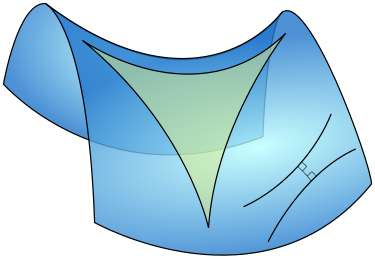
\includegraphics[width=0.3\textwidth]{figs/Hyperbolic_triangle.png}    
    \caption{Section of a hyperbolic space.}
    \label{fig:hyperbolicSpace}
\end{figure}


